\section[第6章\q 好习惯胜过列预算]{第6章\\ 好习惯胜过列预算}
\label{sec:ch6}

周四早上，外头有点冷，尽管柔伊裹紧了大衣，走在风中还是觉得冷到骨子里头去了。她在要进入海伦娜咖啡听时，犹豫了一下。杰弗瑞说的话言犹在耳。她虽然不喜欢他的愤世嫉俗，但他说的也有几分道理，不是吗？或许，她可以进去略作停留，然后就去上班。

她深吸一口气，推门进去。

她发现亨利坐在角落的高脚椅上，坐在他对面和他说话的高个子男人打扮非常牛仔风：打着领结，烫得硬挺的衬衫，黑色的牛仔裤，蛇皮靴，脸像内华达山脉一样饱经风霜。

排队等着买拿铁时，柔伊不禁想到，亨利坐在那张桌子的神情，好像这里是他的办公室。突然有个念头闪过柔伊的脑子，或许亨利不是咖啡师，而是早班经理。但芭芭拉不是说他是咖啡师吗？

\subsection{编列预算对个人一点都不管用}

“早安啊，柔伊。”看到柔伊拿着拿铁走过来，亨利招呼道：“这位是我朋友，拜伦，在能源产业做事。”

“我叫本·唐森。”男人说，上前来和柔伊握了手。“可是我的朋友都叫我拜伦。不过我的冤家都在奥克拉荷马州，所以也不在乎别人怎么叫我。”

“很高兴认识你，拜伦。我是柔伊‧丹尼斯。”柔伊也握住了他的手。如果说亨利的手好像一款精致的油画布，拜伦的手则像水牛皮。“希望我没有打扰你们。”柔伊说。

“没有的事。”亨利说，对着一张空座椅示意着。“请坐。柔伊也喜欢漂亮的摄影照片。”柔伊在凳子落坐时，亨利对拜伦介绍说。

“亨利也分享了他的理财洞见。”柔伊说。

拜伦眉头皱了起来。他缓缓点头，说道：“喔。就是那三个秘密？首先付钱给自己？”

“正是。”柔伊说：“致富很简单，每天10美元。”她笑着回答。

拜伦又皱起眉头。“哎，”他叹气说：“你这个咖啡小子，给小女孩灌输了什么？”

亨利笑着朝拜伦靠过去。“其实她已经很富有了，只是她不知道。”亨利自信的说，又朝柔伊微笑着。

“哇，”柔伊说，“还真高兴现在知道了。”

拜伦咯咯笑着。

亨利低头，看着柔伊说：“虽然你也遇到了一个难题。”

不是一个，是好几个。柔伊说：“很大的难题。碰到理财的事，我就成了麻瓜。”

亨利点头。柔伊继续说：“坦白说，我很难运行什么理财方案。我理解‘先付钱给自己’的点子。但是我不觉得自己可能在日复一日、年复一年的生活中，实际落实这一做法。”

亨利点头。“你可能是做不到。那就是为什么还需要第二个秘密了。”他停顿一下，让他们的思路跟上来。“我猜想，你一定听说过罗列预算的种种好处。”

柔伊心想，喔，老天，还真戳中要害了。柔伊最讨厌预算，虽然她知道这才是理性的做法，但有时候，她就是不愿意做。

“预算。”拜伦大声说：“哈。写预算时，你好像已经统揽全局，写完后，就是和其他垃圾一起丢进废纸篓的下场。”

柔伊忍不住大笑起来。看来这个拜伦与她是同一国的。

拜伦还没有就此停止。他继续说：“预算，什么鬼啊？”说到激动处，他弯下身子，对着柔伊：“你刚说你讨厌预算，对吗？”柔伊点头。

“那最正常不过了，因为每个人都讨厌预算。好啦，也不是每一个人啦！也有少数人，他们天性就喜欢预算。这群人简直好像独角兽一样稀奇。我们需要这样的稀罕人类，所以让他们身居要职。在我工作的地方，就有一个，他是财务首席执行官。我想，他可能枕头底下都放着一张预算表。我们其他人都是平凡之人。我们讨厌这种事情，避之如毒药。”

柔伊倒是好奇，儒雅的咖啡师对这样率直的言论作何反应。

亨利只是点着头说：“他说的没错。”

柔伊看着亨利说：“啊？什么？”

“编列预算对企业或其他组织机构来说，成效不错。”亨利继续说：“但对我们个人来说，效果不佳。如果需要列出每周支出预算表来存点钱，那几乎是不可能的事。不是哪一个人的问题，是人性如此。\textbf{个人的支出预算看似有理，其实是行不通的}。”

“你知道为什么会这样吗？”拜伦问。

柔伊清了清喉咙，说：“不知道。为什么？”

“因为很无趣，这就是原因。”拜伦又开始长篇大论起来，“就像节食一样，知易行难。清楚想好钱要用在哪里，然后把生活压缩到针孔那么小，简直是恶梦。不如顺应天性，想怎样生活就怎样生活吧！”

亨利笑说：“这话确实没错。这也多少正是我要提出‘先付钱给自己’一说的原因。虽然听似荒唐，却是最可能行之有效的办法。”

他把笔记本翻到昨天打开的那一页，在“先付钱给自己”的下方，写上：

{\kaishu 2.不做预算，而是养成习惯}

“如果强迫自己每周写1张支票，或在在线完成存款，早晚会不想做的。没什么原因，就是不想去做。”

“柔伊，我问你，你觉得自己很忙吗？”

“是。”柔伊回答，“保守一点来说，今年工作都满了。”

亨利点头。“那也是理所当然的。每个人都很忙。我想，要你再多列一个周预算，然后照着预算生活，大概是最不可能的任务了。虽然，事实可能是你就不想做这件事。”

这点柔伊没有异议。

“唯一的办法，”亨利说：“就是把这些每天都需要去做的事，设置成一个自动系统，让它们自己完成。就不需要纪律、自律，或者什么意志力了。就是设置，然后完成。”

“不在口袋里的钱，就不要花。”拜伦说。

“这就是了。”亨利说：“这就是自动体系的完美。不管隔周，还是每周，或是每月，每次拿薪水的时候，就会有钱自动转到401帐户去，甚至还在交税之前。就是类似的道理。”

“这么简单？”柔伊问。

“必须这么简单啊！如果不够简单，就会坚持不下去。如果没有变成自动的，也不可能坚持下去。”

“设成自动完成。”柔伊嘀咕着，把字打进手机。

\subsection{设置帐户自动化，才能有效储蓄与投资}

拜伦又开口了。“这个政策政府也是花了好长时间才想出来的。直到二战时，我们富裕的美国人赚到了总是先放在自己口袋，然后第二年才交税给政府。问题就在，我们富裕的美国人不太会计划，不列预算。”他笑着说：“因此政府花了很多力气，教我们如何省着花，次年可以有钱交税。然后，战争后的出生那一代，一样没有改善。因此，美国政府老大想到‘用这套体系，简单就可以收到税’。”

“自动。”亨利补充说。

“自动的。”拜伦重复一遍，“在薪水还没到达没纪律的小手里前，就先自动扣款了。而且，你知道吗，竟然有效。我们每赚1美元，政府都先课到了税。”

“然后公司企业加入到这个游戏中来。”亨利说。“你有参加过哪家健身房的会员吗，柔伊？”

柔伊是健身房会员，她会去使用跑步机和其他设备。

“他们是不是每个月从你的帐户自动扣除会费？”

柔伊点头同意。“我参加时，他们就这样设置的。”

“没错！”拜伦说：“现在许多公司都这样，因为这招有效。”

“所以这就是第二个秘密了。”亨利说：“只要对自己也这样，就可以了。其实政府也对你做了同样的事，在他们收税前就先为你做了一件事。”

“我的401退休帐户？”柔伊嘀咕。

“是的，你的退休金帐户。”亨利同意说：“也就是税前退休金帐户。还有其他类似的计划，比方说自雇者的SEP退休金制度，其他国家也有其他的名称。虽然名字不同，有一个细节却是一样的，\textbf{就是在交所得税之前，先存钱养自己的老}。”

“说到这个，”拜伦说着，把座椅往后推了，站起身来。“女士、先生，我觉得这个时候该配上海伦娜的好点心。这位女士，喜欢什么？”

柔伊微笑着说：“我不饿，谢谢！”她已经忘记了上一回被称作女士是什么时候了。

“你朋友和你一样，老派优雅。”柔伊和亨利看着拜伦走去柜台拿点心。

“没错。”亨利说：“而且百折不挠。拜伦过去在石油产业做事，现在那个产业时机不好。后来来纽约，找到了现在的工作，在一家公司的能源部门研究可再生能源：风力、太阳能，还有其他新科技。非常有趣。还有氢能源，废弃的热能再利用……”他加重了语气。“我老爸那一代，都没听说过的新玩意。”

柔伊笑了起来。她对拜伦的印象还真不错。

“欢迎来到未来社会。”亨利补充一句。他又看着柔伊说：“但是，你依然有疑问。”

“是的。”柔伊说。“我想，疑问还不止一个。”

“没关系，我们来讨论。”

柔伊想说，讨论当然好。但柔伊不想出口伤人，但是她不知道如果不开口说出来，杰弗瑞的疑问就会一直留在她脑中。

“就是，昨天，”她开口，亨利点头。“你提到把收入的部分拿出来，放到另一个帐户，1年赚到10％利息。”亨利又点头，“这点我不理解。我的一个朋友说，现在是不可能有10％利息，那是过去的行情了。”

亨利笑了。“我了解。许多人都对此持怀疑态度。可是事实是，从1926年之后，他们开始有可靠的数据纪录之后，股市每年的平均获利率超过10％。当然，经济景气时好时坏，有熊市、有牛市。收入多少还与时间点有关，也和投入哪个企业有关。但是去除个别例外事件，从大局来看，平均成长还是在10％以上。市场有时起，有时落，但是落了之后，通常还是会起来。没有哪个市场是跌了之后，就再也不起来的。”

“2008年金融海啸之后，大家都说赚钱的时机已经过去了。猜猜，后来的市场行情？”

“又起来了？”柔伊问。

亨利点头同意：“平均年获利超过10％。”

“哇！”柔伊惊呼。

“从过去的历史来看，”亨利说：“最保守的估计，股市债券的获利也在8％以上。不过，具体数字不是重点。重点是，存钱，复利让钱生出钱来。”

“嗯哼！”柔伊回想着和杰弗瑞的对话，“可是即便我取出部分收入到另一个帐户，政府还是要课所得税的，不是吗？不管我放在原本的薪水户头，或另外的户头？”

“这点没错。但如果可以多存一点，而不是把收入的30\%交税给政府，你手上会有更多现金，可用于投资。时间和复利会让你更有余裕。这些生出来的钱，不用缴税。”说着，亨利翻开了笔记本新的一页。“这里，我来画给你看。”

亨利画出一张图表，上面有两条上升的曲线，还标注了一些数据。

前方柜台处爆发出一阵笑声。柔伊抬头看了看，看到拜伦正在和其他客人聊天，他说了一个笑话还是什么。他们大笑着，柜台后方的工作人员也跟着一起笑。

亨利不受这些声音的影响，解释他画出的图表。

“我们举例来说，你每年投入1万美元在投资上，30年后，这笔钱会变成66.1万美元。但如果你把这笔钱放到一个延后缴税的帐户上，同样金额，同样时间，金额会超过170万。也就是说，3倍之多。”

柔伊无法核实具体数字细节，但她看得出大数据。“没错，近3倍。”

\begin{figure}[htbp]
    \centering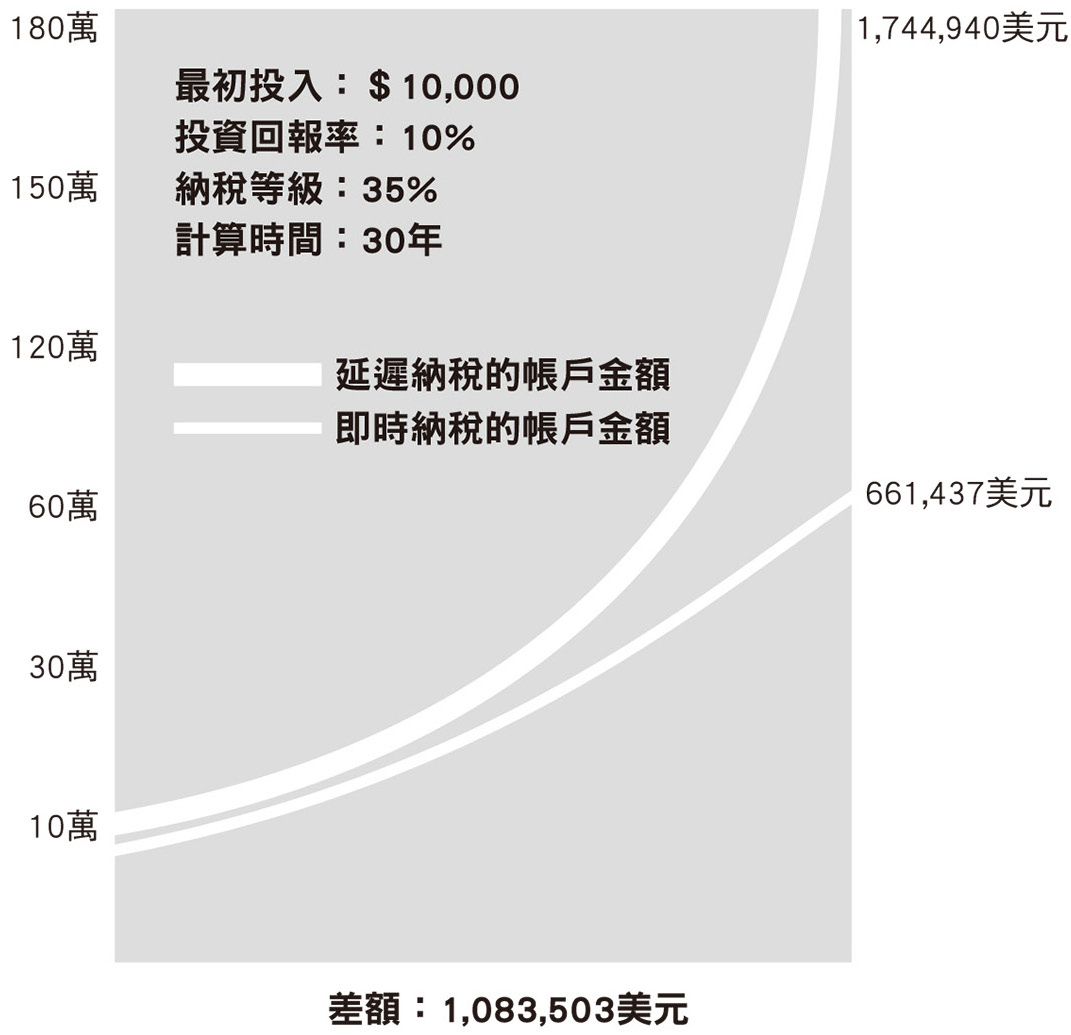
\includegraphics[width=0.7\linewidth]{images/B-95.jpg}
    \caption{延后缴税账户大不同}
\end{figure}

“是的，如果不先缴税，就可以照着这条曲线成长。”亨利解释：“金额快速成长。我不是叫你不要缴税，只是延后缴税。如果你实在想先缴税，建议可以开一个罗斯IRA帐号，那里产生的收入是不用课税的，因为进去的钱原本就已经缴过税了。但是如果让我在先保有现金，之后再交税给政府；和先缴钱给政府，然后再存现金之间做选择，我当然先存现金，再缴税。你当然可以有自己的选择。”

柔伊盯着看了很久。“这个道理不是人人都该知道的吗？”

亨利耸耸肩膀。“这是个好问题。有时候，最直白的道理反而容易被忽略。或者，被认为太简单，不需要再解释或者推广。不值得多说。”

“你知道有个问题，叫做如何吃掉一头大象吗？”

柔伊喝了一口咖啡。“一次吃一点。”

“\textbf{这也正是累积财富的办法。一次存一点}。但是大多数人认为累积财富的办法是中个乐透之类的。比方说，特别幸运的有个好朋友，因为虚拟电子货币给了你一笔酬金，或者买了一支别人不知道的科技绩优股。”

柔伊想起杰弗瑞想要发明下个Instagram运用程序的梦想。

“或者说继承大笔遗产啊、或有架钢琴打中了有钱的姨妈。”这家伙记性还真好，柔伊想着，笑了出来。

“或者在自家后院挖到宝藏。你知道这些的相同点吗？虽然版本不同，但其实都只是某天我走运了的不同说法。”

“这在电影里会发生，但是现实中呢？”亨利摇了摇头，“在中了乐透的背后，有无数个没中奖的购买者。做着发财梦的人成千上万，但是那不过是神话。用一个奇迹来安慰自己，从而不用面对日复一日的寻常日子。”

“没错。”柔伊回答：“你让那些说词都显得空洞无力。”

“因为这些话原本就没有说服力啊！这样的理财法，有如美国诗人梭罗所言‘在死寂的绝望中过活’。”

“但关键是，事情是可以改变的。柔伊，你的命运之船就在此地，就在你脚下。你站在船坞上，船儿将出港。你是船长。”

“问题是你想要打开怎样的行程？你想去哪里？”

“来啰！”拜伦的声音响了起来，他回到桌边，端着一个大盘子，里头有两块厚片蛋糕，旁边还有一杯咖啡，他把咖啡放到柔伊前方。“栉瓜派。拿铁是给柔伊的，说不定你想续一杯。”

亨利看了看在柜台前长长的点餐人群，他起了身。

“不好意思。我要过去了。”说完，他就朝柜台后方走去。

拜伦从一旁桌子的托盘上又拿来一杯热饮，也是刚买的。“热呼呼的义式浓缩咖啡，黑咖啡，为了——”
